\documentclass{article}[18pt]
\ProvidesPackage{format}
%Page setup
\usepackage[utf8]{inputenc}
\usepackage[margin=0.7in]{geometry}
\usepackage{parselines} 
\usepackage[english]{babel}
\usepackage{fancyhdr}
\usepackage{titlesec}
\hyphenpenalty=10000

\pagestyle{fancy}
\fancyhf{}
\rhead{Sam Robbins}
\rfoot{Page \thepage}

%Characters
\usepackage{amsmath}
\usepackage{amssymb}
\usepackage{gensymb}
\newcommand{\R}{\mathbb{R}}

%Diagrams
\usepackage{pgfplots}
\usepackage{graphicx}
\usepackage{tabularx}
\usepackage{relsize}
\pgfplotsset{width=10cm,compat=1.9}
\usepackage{float}

%Length Setting
\titlespacing\section{0pt}{14pt plus 4pt minus 2pt}{0pt plus 2pt minus 2pt}
\newlength\tindent
\setlength{\tindent}{\parindent}
\setlength{\parindent}{0pt}
\renewcommand{\indent}{\hspace*{\tindent}}

%Programming Font
\usepackage{courier}
\usepackage{listings}
\usepackage{pxfonts}

%Lists
\usepackage{enumerate}
\usepackage{enumitem}

% Networks Macro
\usepackage{tikz}


% Commands for files converted using pandoc
\providecommand{\tightlist}{%
	\setlength{\itemsep}{0pt}\setlength{\parskip}{0pt}}
\usepackage{hyperref}

% Get nice commands for floor and ceil
\usepackage{mathtools}
\DeclarePairedDelimiter{\ceil}{\lceil}{\rceil}
\DeclarePairedDelimiter{\floor}{\lfloor}{\rfloor}

% Allow itemize to go up to 20 levels deep (just change the number if you need more you madman)
\usepackage{enumitem}
\setlistdepth{20}
\renewlist{itemize}{itemize}{20}

% initially, use dots for all levels
\setlist[itemize]{label=$\cdot$}

% customize the first 3 levels
\setlist[itemize,1]{label=\textbullet}
\setlist[itemize,2]{label=--}
\setlist[itemize,3]{label=*}

% Definition and Important Stuff
% Important stuff
\usepackage[framemethod=TikZ]{mdframed}

\newcounter{theo}[section]\setcounter{theo}{0}
\renewcommand{\thetheo}{\arabic{section}.\arabic{theo}}
\newenvironment{important}[1][]{%
	\refstepcounter{theo}%
	\ifstrempty{#1}%
	{\mdfsetup{%
			frametitle={%
				\tikz[baseline=(current bounding box.east),outer sep=0pt]
				\node[anchor=east,rectangle,fill=red!50]
				{\strut Important};}}
	}%
	{\mdfsetup{%
			frametitle={%
				\tikz[baseline=(current bounding box.east),outer sep=0pt]
				\node[anchor=east,rectangle,fill=red!50]
				{\strut Important:~#1};}}%
	}%
	\mdfsetup{innertopmargin=10pt,linecolor=red!50,%
		linewidth=2pt,topline=true,%
		frametitleaboveskip=\dimexpr-\ht\strutbox\relax
	}
	\begin{mdframed}[]\relax%
		\centering
		}{\end{mdframed}}



\newcounter{lem}[section]\setcounter{lem}{0}
\renewcommand{\thelem}{\arabic{section}.\arabic{lem}}
\newenvironment{defin}[1][]{%
	\refstepcounter{lem}%
	\ifstrempty{#1}%
	{\mdfsetup{%
			frametitle={%
				\tikz[baseline=(current bounding box.east),outer sep=0pt]
				\node[anchor=east,rectangle,fill=blue!20]
				{\strut Definition};}}
	}%
	{\mdfsetup{%
			frametitle={%
				\tikz[baseline=(current bounding box.east),outer sep=0pt]
				\node[anchor=east,rectangle,fill=blue!20]
				{\strut Definition:~#1};}}%
	}%
	\mdfsetup{innertopmargin=10pt,linecolor=blue!20,%
		linewidth=2pt,topline=true,%
		frametitleaboveskip=\dimexpr-\ht\strutbox\relax
	}
	\begin{mdframed}[]\relax%
		\centering
		}{\end{mdframed}}
\lhead{CSys}


\begin{document}
\begin{center}
\underline{\huge Timing and Advanced Adders}
\end{center}
\section{Timing}
\begin{itemize}
	\item A buffer doesn't change if an output is high or low, it just makes it either full high or full low
\end{itemize}
In any physical gate or circuit there is a delay between the input changing and the output adjusting appropriately.
\begin{center}
	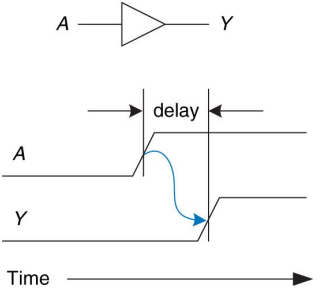
\includegraphics[scale=0.7]{timing}
\end{center}
\begin{itemize}
	\item Note that the lines are not vertical, they rise between low and high
\end{itemize}
\textbf{Propagation delay: $t_{pd}$}: The max delay before the output is stable\\
\textbf{Comtamination delay $t_{cd}$}: The min delay before the output changes
\begin{center}
	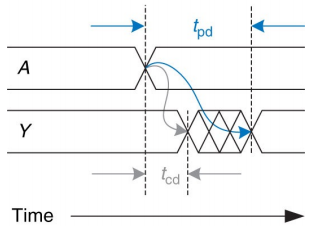
\includegraphics[scale=0.7]{delay}
\end{center}
Delay is caused by:
\begin{itemize}
	\item Capacitance and resistance in a circuit
	\item Speed of light limitation
\end{itemize}
Reasons why $t_{pd}$ and $t_{cd}$ may be different:
\begin{itemize}
	\item Different rising and falling delays
	\item A circuit may have multiple inputs and outputs, some of which are faster than others
	\item Circuits slow down when hot and speed up when cold
\end{itemize}
\section{Critical paths}
\begin{center}
	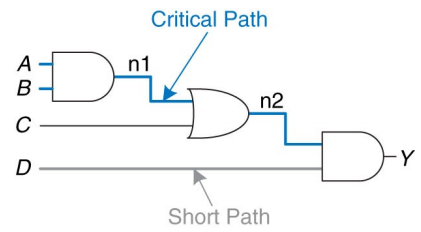
\includegraphics[scale=0.7]{critical_path}
\end{center}
In a circuit the critical path is the path determining the propagation delay of the circuit - i.e. the longest path in the circuit
$$t_{pd}=2t_{pd\_AND}+t_{pd\_OR}$$
The short path is the path determining the contamination delay of the circuit - i.e. the
shortest path in the circuit
$$t_{cd}=t_{cd\_AND}$$
\section{Glitches}
Sometimes the output can temporarily move to an incorrect value before
stabilising.\\
This is called a glitch. 
\begin{center}
	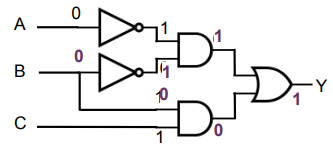
\includegraphics[scale=0.7]{glitch}
\end{center}
With a=0,b=1 and c=1. If b falls to 0, the output will change from 1 to 0 to 1.
\section{Mux delays}
\begin{center}
	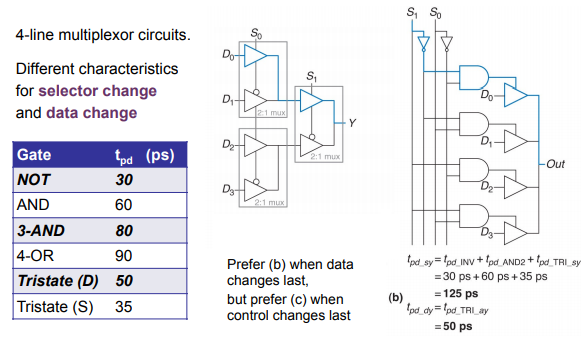
\includegraphics[scale=0.7]{mux_delay}
\end{center}
\begin{itemize}
	\item Tristate D - Data
	\item Tristate S - Selector
	\item The different speeds for different changes need to be taken into account for whatever the use is
\end{itemize}
\section{Adder}
\begin{center}
	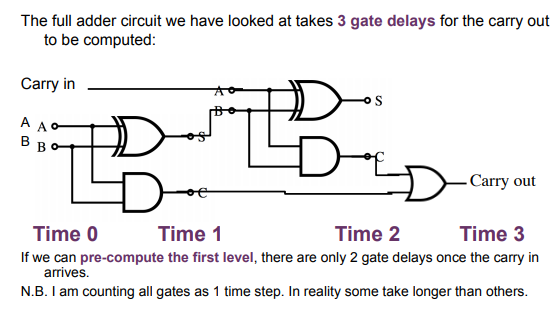
\includegraphics[scale=0.7]{adder}
\end{center}
\section{Ripple adder}
\begin{center}
	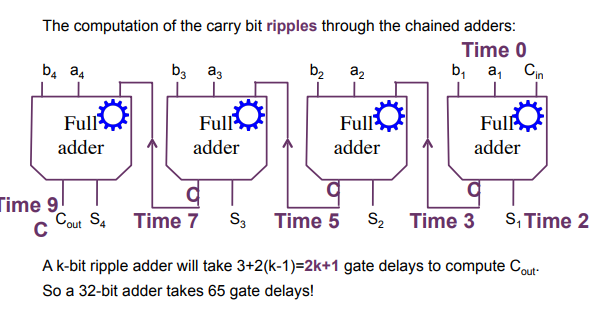
\includegraphics[scale=0.7]{ripple_adder}
\end{center}
\begin{itemize}
	\item 3 time steps for 1st carry, then 2 time steps for each after that as the first level is pre computed
\end{itemize}
\section{Faster Adders - idea}
\begin{center}
	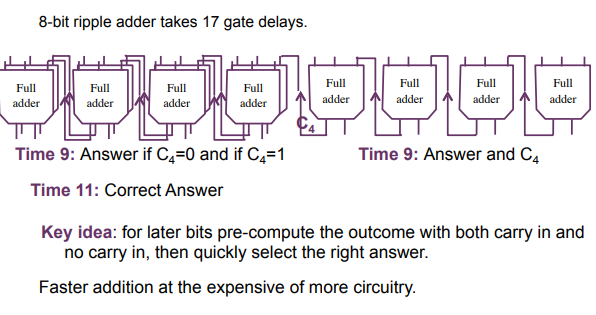
\includegraphics[scale=0.7]{faster_adders}
\end{center}
\begin{itemize}
	\item This uses $c_4$ for the multiplexor and makes large additions much faster, at the expense of more circuitry 
\end{itemize}
\section{Carry-Lookahead Adder}
\begin{center}
	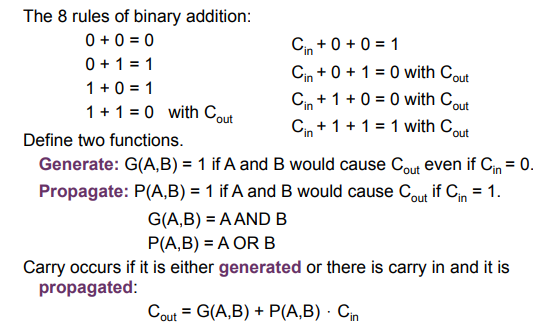
\includegraphics[scale=0.7]{carry-lookahead}
\end{center}
\begin{center}
	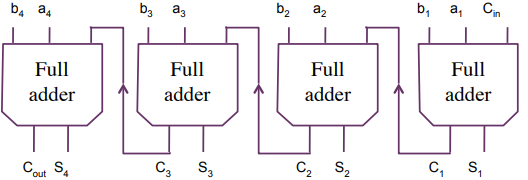
\includegraphics[scale=0.7]{carry-lookahead1}
\end{center}
\begin{center}
	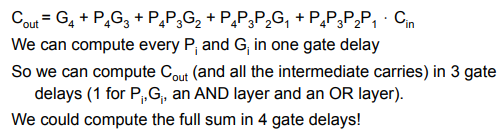
\includegraphics[scale=0.7]{carry-lookahead2}
\end{center}
\begin{center}
	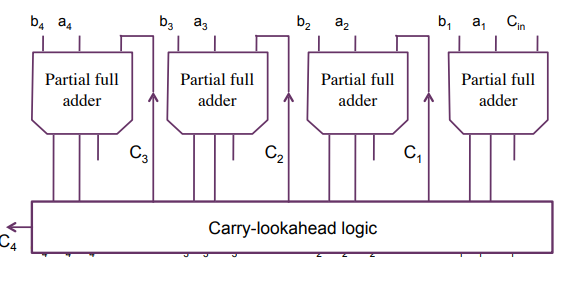
\includegraphics[scale=0.7]{carry-lookahead3}
\end{center}
\section{Partial Full Adder}
\begin{center}
	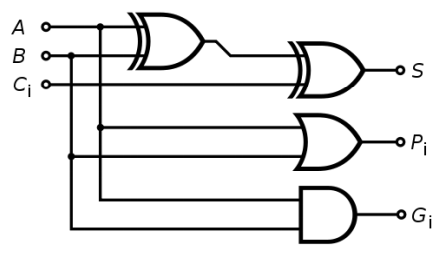
\includegraphics[scale=0.7]{partial_adder}
\end{center}
\section{MSI Chip}
\begin{center}
	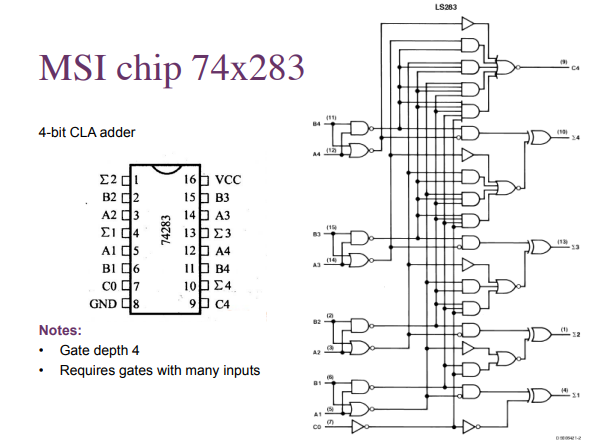
\includegraphics[scale=0.7]{MSI}
\end{center}
\section{More on the carry-lookahead adder}
\begin{center}
	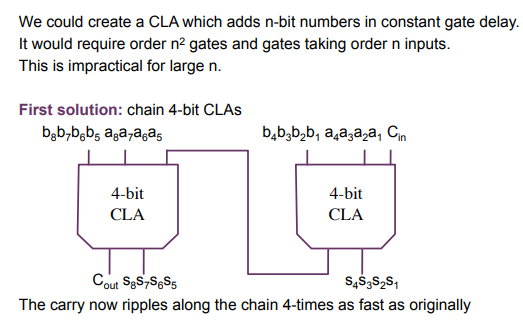
\includegraphics[scale=0.7]{carry-lookahead21}
\end{center}
\section{2 Level Carry-Lookahead Adder}
\begin{center}
	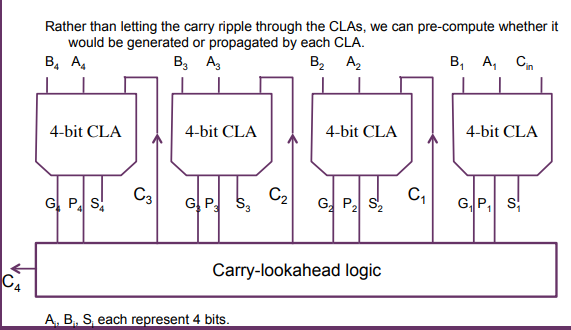
\includegraphics[scale=0.7]{2-level-lookahead}
\end{center}
\begin{center}
	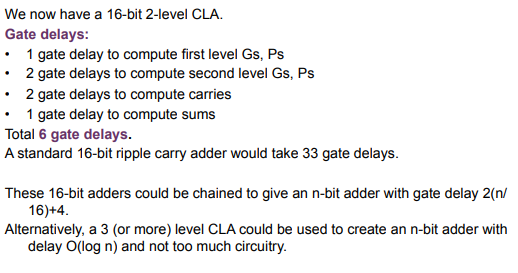
\includegraphics[scale=0.7]{2-level-lookahead1}
\end{center}
\section{Example}
\begin{center}
	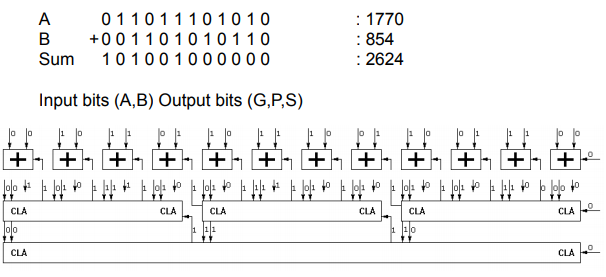
\includegraphics[scale=0.7]{example}
\end{center}
\section{Summary}
\begin{itemize}
	
	\item $t_{pd}$ - propagation delay (time until last answer comes in)
	\item $t_{cd}$ - contamination delay (time before any change)
	\item $t_{pcq}$ - max time until recorded after tick
	\item $t_{ccq}$ - How long before the value is recorded after the tick
	\item $t_{setup}$ - time stable at least this long before tick 
	\item $t_{hold}$ - time stable at least this long after tick
\end{itemize}
\section{Improving clock speed}
\begin{itemize}
	\item Putting registers in allows you to reduce the long delays, allowing a faster clock speed
	\item Work like a production line by separating the jobs
	\item Allows 1st half to work on next calculation while 2nd half is working on the end of the calculation
	\item First half takes less time than all of previous one, allowing for a faster clock speed
	\item So overall a calculation takes 2 clock ticks, so the latency will be larger, but the time for a large number of calculations will reduce drastically
	\item If you keep adding registers it keeps getting better, but the resources required mean that you get diminishing returns
\end{itemize}

\end{document}